\documentclass[twoside]{report}
%\usepackage[a4paper, total={6in, 8in}]{geometry}

%%%%% ADDED TO SUPPORT TT BOLD FACES %%%%
\DeclareFontShape{OT1}{cmtt}{bx}{n}{<5><6><7><8><9><10><10.95><12><14.4><17.28><20.74><24.88>cmttb10}{}
\renewcommand{\ttdefault}{pcr}
%%%%% END %%%%%%%%%%%%%%%%%%%%%%%%%%%%%%%
\usepackage{atbegshi,picture}
\AtBeginShipout{\AtBeginShipoutUpperLeft{%
  \put(\dimexpr\paperwidth-1cm\relax,-1.5cm){\makebox[0pt][r]{
\includegraphics[width=3cm]{figs/inno.jpg}}}%
}}

\usepackage[english]{babel}
\usepackage{blindtext}

\newenvironment{bottompar}{\par\vspace*{\fill}}{\clearpage}

\usepackage{amsmath,amsfonts}

\usepackage{amsthm}
\newtheorem{theorem}{Theorem}
\newtheorem{corollary}{Corollary}
\newtheorem{lemma}{Lemma}
\newtheorem{proposition}{Proposition}
\theoremstyle{definition}
\newtheorem{definition}{Definition}
\theoremstyle{remark}
\newtheorem*{remark}{Remark}
\theoremstyle{remark}
\newtheorem*{example}{Example}

\usepackage{float}
\usepackage{graphicx}
\usepackage{array}
\usepackage{multirow,array}
\usepackage{caption}
\usepackage{subcaption}
\usepackage{paralist}
\usepackage{listings}
\usepackage{zed-csp}
\usepackage{fancyheadings}
\usepackage{color}

\usepackage{upgreek}
\usepackage{bm}
\usepackage{hyperref}
\usepackage{setspace}
\usepackage{booktabs}
\usepackage{multirow}
\usepackage{longtable}
\usepackage[font=singlespacing, labelfont=bf]{caption}
\usepackage[parfill]{parskip}

\usepackage[utf8]{inputenc}
\usepackage{makecell}

\usepackage{minted}

\usepackage[%
backend=bibtex      % biber or bibtex
%,style=authoryear    % Alphabeticalsch
,style=numeric-comp  % numerical-compressed
,sorting=none        % no sorting
,sortcites=true      % some other example options ...
,block=none
,indexing=false
,citereset=none
,isbn=true
,url=true
,doi=true            % prints doi
,natbib=true         % if you need natbib functions
]{biblatex}

\bibliography{IEEEabrv,thesis}

\usepackage{enumitem}
\newlist{inlinelist}{enumerate*}{1}
\setlist*[inlinelist,1]{%
  label=(\arabic*),
}

\pagestyle{fancyplain}

\usepackage{titlesec}
% \topskip 50pt
\titleformat{\chapter}[display]{\normalfont\huge\bfseries}{\chaptertitlename\ \thechapter}{20pt}{\Huge}
\titlespacing*{\chapter}{0pt}{0pt}{40pt}

% remember section title
\renewcommand{\chaptermark}[1]%
	{\markboth{\chaptername~\thechapter~--~#1}{}}

% subsection number and title
\renewcommand{\sectionmark}[1]%
	{\markright{\thesection\ #1}}

\rhead[\fancyplain{}{\bf\leftmark}]%
      {\fancyplain{}{\bf\thepage}}
\lhead[\fancyplain{}{\bf\thepage}]%
      {\fancyplain{}{\bf\rightmark}}
\cfoot{} %bfseries


\newcommand{\dedication}[1]
   {\thispagestyle{empty}

   \begin{flushleft}\raggedleft #1\end{flushleft}
}

\begin{document}\sloppy

\begin{titlepage}

\begin{center}

\textbf{\Large{Modular Language Server: Design and Implementation}}
\vspace{4cm}

\textbf{\Large Innopolis University} \\

\vspace{0.60cm}

{\Large Thesis submitted to The Innopolis University in conformity with the
requirements for the degree of Bachelor of Science.}

\vspace{6cm}

{\Large presented by}

\vspace{0.40cm}

\textbf{\Large Mike Lubinets}
\vspace{0.40cm}

{\Large supervised by}\\
\vspace{0.40cm}
{\bf\Large Eugene Zouev}\\
\vspace{0.60cm}
{\Large 12/20/2017}


\end{center}
\end{titlepage}

\newpage
\thispagestyle{empty}

\mbox{}

\vspace{7cm}

\begin{flushright}

\textbf{\LARGE Language Server implementation for SLang}

\vspace{0.1cm}

\rule{\linewidth}{0.15cm}%
\end{flushright}

\newpage
\setcounter{page}{5}

\newpage
\thispagestyle{empty}
\mbox{}
\newpage

\tableofcontents
%\listoftables
%\listoffigures

\newpage
\begin{abstract}
На сегодняшний день у нас есть много зрелых инструментов и интегрированных сред разработки для набора широко используемых языков программирования.
Эти инструменты развивались в течении многих лет для удовлетворения большинства потребностей индустрии разработки программного обеспечения.

Однако такие программные продукты зачастую очень сложны и имеют монолитную архитектуру, обычно автономную
от инфраструктуры компилятора языка, что затрудняет замену ключевых компонентов или реализацию поддержки дополнительных языков.

В этой работе мы увидим как строилась архитектура компиляторов и какие осложнения это вызывает в современных реализациях IDE, 
современый подход к построению компиляторов и реализацию гибкой
распределеной интегрированная среды разработки на основе концепции Language Server для мультипарадигменного языка программирования SLang\cite{Zouev2017}.
\end{abstract}

\chapter{Introduction}
\label{chap:intro}
\chaptermark{First chapter heading}

Nowadays we have a lot of mature toolkits and integrated development environments for a set of widely used programming languages
evolved through years to fulfill needs of the most of software development industry.

However, such software products are highly complex and often have a monolithyc archithecture, usually standalone 
from the language compiler infastructure which makes it hard to replace key components or implement support for additional languages.

In this paper we will see how conventional compilers have been archithectured and what complications 
this consequently brought to modern IDE implementations, review the modern approach to compiler construction and implement a flexible 
distributed integrated development environment with the \\Language Server Protocol, for a multiparadigm SLang\cite{Zouev2017} programming language. 
\chapter{Literature Review}
\label{chap:lr}
\chaptermark{Second Chapter Heading}

\section{Conventional compilers in the modern world}
\label{sec:review_1}

Since the middle of $20^{th}$ century researchers and the industry have done a great
work in compilers development focusing on the main goal of classic compilation
problem: producing fast and effective object code for execution on a virtual
machine or a microprocessor.


However, the other compilers’ capability as developer’s code inspection
instruments able of providing comprehensive information of code semantics
remains uncommon and rarely well-developed in the modern compilers of
popular programming languages.


The most common illustration of this problem can be found in an average Java
developer’s set of instruments:

Java code is usually compiled with Sun Java Compiler, which, “being a
monolithic program, constructed as a ‘black box’”\cite{Zouev2005}, can only accept the input
code and produce optimized JVM byte code.
\newpage
Yet a modern development environment includes a set of tools for
programming assistance and requires advanced language syntax and
semantics inspection, which is not possible without building a Semantic
Representation\cite{Zouev2005}. To build it one needs to reimplement core functionality of a
compiler.


It’s easy to understand the very reason of the issue looking back to the past:
traditionally programs have been considered as mere text objects to be
converted into an executable code. According to this assumption, compilers
were designed in a very logical way: they haven’t maintained any semantic
representation of source code, only some low-level internal IR.


These compilers’ IRs have very limited set of use cases\cite{Zouev2005, Zouev2010}, moreover they are
good for the only task: object code generation for several microprocessor
architectures. Also compiler’s IR is not stable and tends to change very actively
during compiler development\cite{FreeSoftwareFoundation2016}. Hence the internal compiler’s IR can’t really
be used to build good and reliable development tools.


The situation is even more frustrating with C++ tooling: the language syntax
and semantics is a lot more complicated than Java’s, so building a custom
compiler is a very complex task.

As a result, there is a notable lack of instruments for C++\cite{Zouev2010}, and existing
ones are pretty sophisticated: JetBrains CLion IDE implements its own parser
and semantic analyzer to build auto-completion, refactoring and static analysis
tools upon their own C++ SR. Being a complex software product, CLion’s parser
tends to have its own misfeatures and a few month implementational lag to
fully adapt for new standards.


Microsoft Visual Studio “suffers” from this too: VC++ generates IR that is useful
only for code generation: it is fragmented and very low-level.
The C\&C++ IntelliSense tooling in Microsoft Visual Studio IDE is implemented
as a solution separate from VC++ compiler.

\newpage

\section{Modern compilers and SR: \\a new hope}
\label{sec:review_2}

In spite of the fact that traditional compilers are widely used today, their lack of
IDE integration capabilities were realized long ago and currently a lot of new
languages are aiming to implement a Semantic Representation as a stable IR
shared with external tools.

Following \cite{Zouev2005, Zouev2010}, unlike a traditional compiler IR, Semantic Representation contains a full
knowledge of a program, including the aspects that are implicit in the source
code. This trait enables some pretty powerful opportunities based on
semantics analysis:

\begin{itemize}
    \item Code generation
    \item Distributed (or recursive) Validation
    \item Human understandable visualization
    \item Static analysis
    \item Program interpretation
    \item Semantic Search: the very powerful technique of querying code semantic objects (“find all classes derived from class C that do not override the virtual function f”)    
\end{itemize}

There are two main ways to represent an SR and share it with SR clients: to
provide an access API operating on an SR (proprietary) binary format \cite{Cannon, FreeSoftwareFoundation2016},
relational database representing a software structure \cite{Linton1983}, or to output SR as an
open textual format\cite{TheRustTeam2016}.

“Generally speaking, API is a universal way to implement any required
functionality, however with changing requirements it’s impossible to predict a
spectrum of clients’ needs”.\\
And an open SP format can be a solution to potential problems: “open formats
usually have a lot of access means: from simple APIs to high level specialized
products. Besides, it’s possible to implement one’s own interfaces to process SR
represented with open format”.\cite{Zouev2005}

A particular format may be something self-designed[7] or a standardized
solution such as XML\cite{Germon}, or JSON\cite{ECMA-4042013}, as an altetnative.

\section{LSP and distributed approach to building development
environment}
\label{sec:review_3}

Considering the things discussed above, nowadays we have a solid basis to
provide a good tooling based on semantic analysis: methods to represent
software source code’s Semantic Representation and evaluate it accordingly to
clients’ needs.

Modern IDEs apply those methods to deliver a decent service, but still there is a
problem: those software products use their own implementations of compilers,
usually proprietary and unrelated to the original language’s development team.
It implies a set of problems noted in the \ref{sec:review_1}.

Having a good modern compiler capable of generating an SR makes things a bit
less complicated but still doesn’t solve the language-specific IDE
implementation time and cost problem.

Obviously, these problems are not unique for the IDE class of products, but for
any big monolithic architecture, and the solution may be pretty straightforward:
if we can lower the bonding of the system and represent a development
environment as a set of tools instead of one integrated solution, we can
distribute the IDE implementation to have a set of disjointed modules:
\begin{itemize}
    \item An editor
    \item Compiler to SR
    \item SR clients (described in \ref{sec:review_1})
    \item Protocol between an editor and the language-specific part
\end{itemize}

\newpage

\begin{figure}[H]
    \centering
    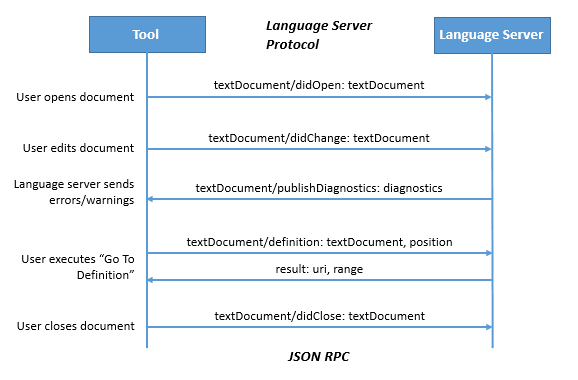
\includegraphics[width=1.0\textwidth]{figs/lsp.png}
    \caption{Language Server Protocol}
\end{figure}

The last one have not been introduced yet: the protocol to connect any
third-party tool to the language infrastructure, achieving a decent IDE-like
functionality without its maintenance and development costs
   
Language Server and Language Server Protocol introduced by Microsoft in 2016
represent a development environment as two disjoint parties:
\begin{itemize}
    \item Language Servers to implement all the SR analysis things
    \item Clients as editors or other devtools using the LSP to communicate with Language Servers \cite{Sourcegraph}
\end{itemize}

\newpage
\section{Conclusion}
\label{sec:review_conclusion}

Conventional compilers with a monolithic architecture, that are only good at executable code generation,
are hard to integrate into a modern development environment as they do not share 
semantic representation of the source code, thus to develop a good IDE one must write his own 
source code to Semantic Representation compiler.

The modern compiler (that do share a high-level intermediate representation) is
a big step towards simpler language toolings and it can become even more convenient
combined with a distributed IDE architecture that splits an editor and the language toolchain
into two sparce parts, linking them via a standardized protocol.

This approach gives language developers a great opportunity to make use of an
existing development infrastructure, providing their Language Server for a
giant set of development tools, as well as a way to fearlessly experiment with new and
existing analysis techniques, e.g. a Software Knowledge Base\cite{Wanghong}, described by
Bertrand Meyer, may be implemented as a language server module, as an
alternative approach to the one selected by the original author in 1985:
integration of analysis tool into an editor was not possible back then, but this is
the exact thing that LSP is good for now.

Concluding, the Language Server may be considered to be the most feasible
solution to rapidly bootstrap rich development infrastructure for aspiring new
languages, with a broad path to evolve further.
\chapter{Methodology}
\label{chap:met}

\section{SLang Semantic Representation Design}
\label{sec:met:ir_design}
Waiting for the SR meeting results

\section{Compiler integration}
\label{sec:met:ls_compiler_interop}
The Language Server idea is to launch the LS instance in the same project directory
opened in the editor, and connect it to the editor via Language Server Protocol.

A Language Server is responsible for language-specific editor features, 
it works on the language Semantic Representation and other metadata 
to perform semantic analysis and consequently provide the editor with usable data in the agreed format via Language Server Protocol.
As Language server heavily relies on the modern compiler, that exposes the SR, 
we need to implement a way to integrate compiler into the Language Server and to enable their inter-operation.

There are two possible ways to achieve that: either to use compiler as a library or invoke it in a separate process, 
feeding specific command line arguments.
\begin{table}[H]
    \centering
    \begin{tabular}{|c|c|}
        \hline
        \textbf{invoking as a command} & \textbf{using compiler as a library} \\
        \hline
        simpler integration & harder integration \\ 
        \hline
        very limited invocation options & complex invocation strategies may be expressed \\
        \hline
        need to (de)serialize data & can exchange binary data \\
        \hline
        need to implement IR traversal in the LS & compiler can expose AST traversal API \\
        \hline
        need to describe compiler internal data types in the LS & compiler can expose internal data types \\
        \hline 
    \end{tabular}
    \caption{Compiler integration methods comparison}
    \label{table:met:compiler_integration}
\end{table}

Since the SLang\cite{Zouev2017} compiler does not expose any AST traversal API or internal data types, most of 
the traits specific to an ``integration as a library" option will not be used in our case.
Moreover, the compiler provides a stable json-formatted SR, which being a text-serialized format, 
can be easily transferred via operating system channel like standard output\cite{TheOpenGroup1997}.

This way, we get a number of convenient features: the compiler can be invoked by our Language Server as a command call, we are not limited 
with any functionality that would require ``compiler as a library" traits, and this option
is easier to implement on both Language Server and compiler ends.
Therefore we can declare this way of integration the most feasible in our case and stick to it.

\begin{figure}[H]
    \centering
    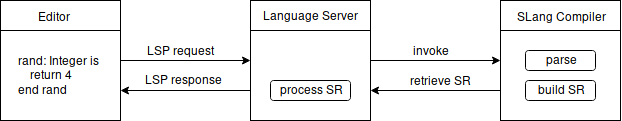
\includegraphics[width=1.0\textwidth]{figs/compiler_integration.png}
    \caption{Workflow with Language Server and integrated compiler}
\end{figure}

\section{Language Server Extensible Architecture}
\label{sec:met:arch}
The main idea of this research is to bring architecture of Language Servers to the next level,
make it modular and extensible, thus allowing third parties to throw in additional functionality for the SLang tooling
with no need to hack into the Language Server code.

Therefore, the architecture of the SLang Language Server is divided into two aggregate components:
\begin{itemize}
    \item The Core
    \item Module System 
\end{itemize}
where the Language Server Core is a framework through which the Modules do operate.

\begin{figure}[H]
    \centering
    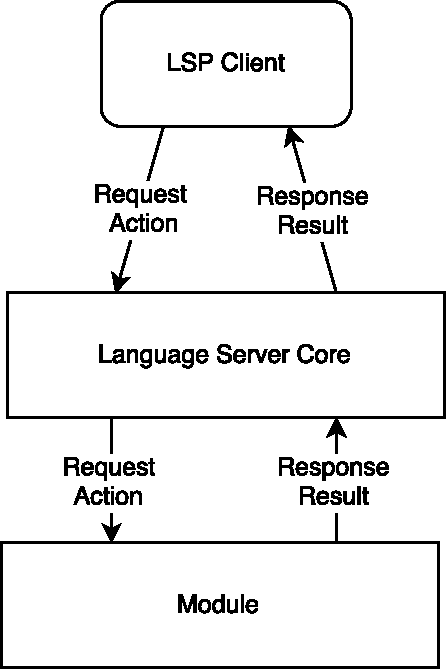
\includegraphics[width=.3\textwidth]{figs/highlevel_architecture.pdf}
    \caption{Language Server High-level Architecture}
\end{figure}

\subsection{Language Server Core}
\label{sec:met:arch:core}
Language Server Core is a basement level of the Language Server on which Language Server Modules will operate.
Responsibilities of LS Core include:
\begin{itemize}
    \item LS Client connection maintenance
    \item Module registry maintenance
    \item Routing of incoming requests and data control flow between modules
\end{itemize}

Each of these responsibilities we shall describe in detail.

\subsubsection{Client connection maintenance}
\label{sec:met:arch:core:connection_maintenance}
According to Language Server Protocol\cite{Sourcegraph}, client controls the lifetime of a server, 
i.e starts it and shuts the server down on demand. After startup, client connects to the server
using one of transports. Since the transport level is not constrained by the LSP, specific transport 
can vary in different implementations.

Language Server Core should support several transports and be able to operate on them to accept requests 
and respond to the client. The list of widely used transports we will implement is
\begin{itemize}
    \item stdin/stdout
    \item tcp
    \item udp
\end{itemize}
Implementing that list will supply the most of LSP clients with an option of how to work with the SLang Language Server.  

\subsubsection{Module Registry}
\label{sec:met:arch:core:module_registry}

To be a foundation for an extensible modular architecture Language Server Core needs to have a subsystem 
for module registering, maintenance and inter-operation organization.

\begin{figure}[H]
    \centering
    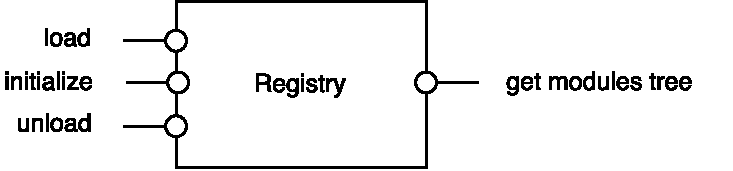
\includegraphics[width=.7\textwidth]{figs/registry.pdf}
    \caption{Module Registry API}
\end{figure}

\newpage
The registry should register and give module status, as well as information on how to launch and connect
internal (core) and external modules. On startup, registry should initialize its state using a predefined directory
containing configuration files. Afterwards, it should maintain an API to load and unload additional modules via LSP.
Consequently, we need to extend the LSP with additional commands for the modules registry:

\begin{itemize}
    \item registryCtl/load
    \item registryCtl/unload
    \item registryCtl/status
\end{itemize}

\subsubsection{Routing and data flow control}
\label{sec:met:arch:core:dispatcher}

After startup, connection setup, module registering and initialization, 
Language Server accepts the first request from the client. 
This request gets validated by Language Server Core, then, after looking up the Module Registry, the request 
gets handed over to the beginning of processing pipeline responsible for handling this type of requests.

Basically the dispatcher part is a glue, that connects all Language Server components together and 
maintains the data flow edges for the modules graph, enabling module inter-operation by the
rules loaded into the Registry and that are discussed further in the section \ref{sec:met:arch:ms}.

There is a simpler alternative approach to module inter-operation organization: let the modules send data 
to each other and organize pipeline as they want. Although peer-to-peer schema here will save a lot of bandwidth, 
it will also inevitably lead to the dependency hell, 
as such approach would require having every module knowing each other and connecting to each other. 
Thus, here we face the classic client/server trade-off: we can offload a ``server" (LS Core) only
if we complicate a ``client" (modules). 
Since the client side is to be developed by third parties, the simpler it is -- the better: 
server, controlling all the data flow, will leave the module developer only with the business logic implementation tasks. 

\subsection{Module System}
\label{sec:met:arch:ms}

Language Server is a great idea to enable IDE-like functionality for
comparably simple text editors, but currently they are mostly designed as 
monolithic software, while their service functions are naturally extensible, 
e.g. it is common for a static analyzer to have modules for different diagnostics.

Similarly, one of Language Server functions is to provide an editor with diagnostics: here we can 
have hierarchy of at least two modules -- the compiler diagnostics and the diagnostics provided by an external static analysis tool.
We can go even further and implement a static analyzer as a base static analysis module and a bunch of atomic diagnostic modules derived 
from this base module. 
The same logic is applicable to every Language Server service to some extent.

Separation of the monolithic core from the actual functionality implemented through modules
will significantly lower the Language Server internal bonding, and will make
module implementation relying on a stable API possible, therefore allowing the core and modules
development to be performed simultaneously with no mutual API breakages.

Therefore another value of an extensible architecture that we can derive is 
Language Server easy adoption for any specific corporate needs. 
As implementing some additional functionality would be as easy as developing a plug-in using 
the Language Server Modules API, corporate users can extend the Language Server 
due to their specific requirements, i.e add custom diagnostics, enforce code style, 
or even hook-up the proprietary static analysis or code generation tools.

\begin{figure}[H]
    \centering
    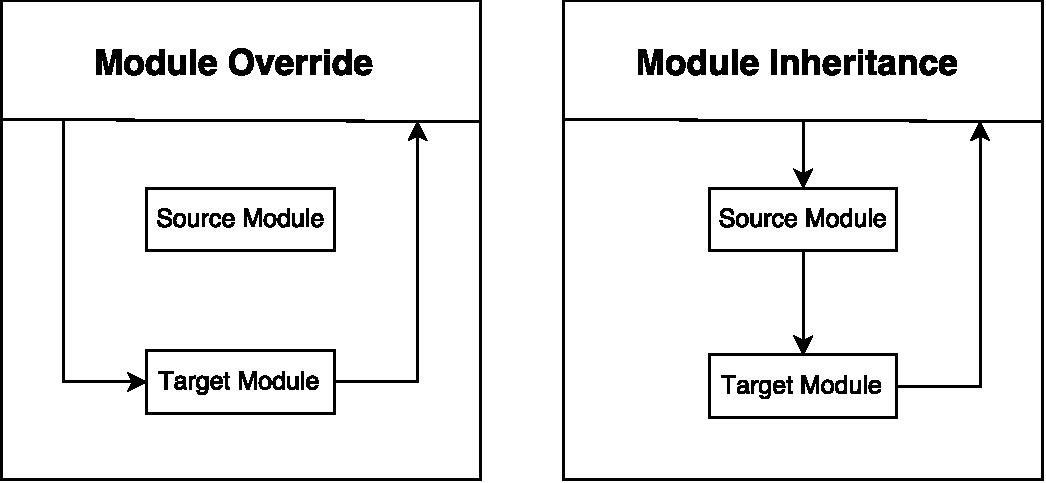
\includegraphics[width=.7\textwidth]{figs/module_hierarchy.pdf}
    \caption{Module Hierarchy}
\end{figure}

One of the ways to develop such architecture was already introduced above: the hierarchy of modules, 
expressed with the basic Object-Oriented Programming terms. In the module hierarchy
modules can either override other modules or extend them in a way of post-processing the
results of base module computation. So the modules would form a classic tree, deriving from a base module,
and intercepting the data flow.

\begin{figure}[H]
    \centering
    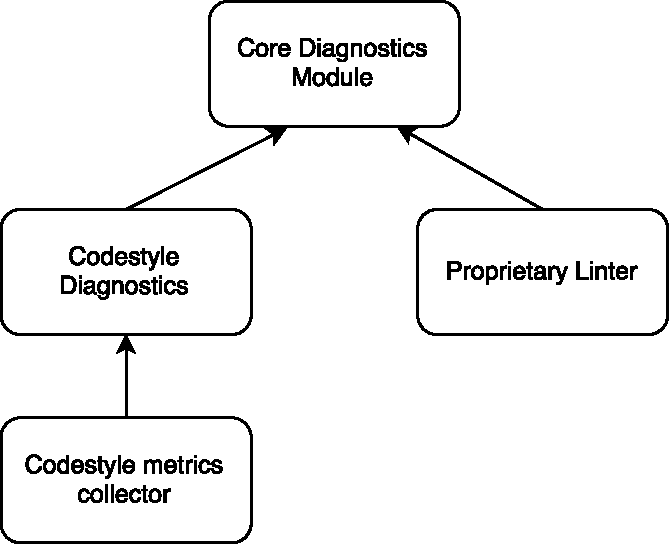
\includegraphics[width=.5\textwidth]{figs/module_tree.pdf}
    \caption{Example Modules Tree}
\end{figure}

Having this as a basement of the modular system architecture, we can derive a 
neat easy-to-use API to build the modules.

In this thesis we have already introduced a notion of the base and derived modules. Taking as an example the modern Object-Oriented languages` 
type systems, we can build a hierarchy with the base modules, distributed bundled with the Language Server, and responsible for
one particular LS Protocol method. These modules will mainly provide the basic run-time for all the derived modules: 
\begin{itemize}
    \item set up data types: the input information, analysis context, and the results.  
    \item perform the construction of the context (if applicable).
    \item intercept analysis results of the derived module and send them to the client through LSP.
\end{itemize}

As one could have figured, it is not really a conventional O-O paradigm inheritance model: core modules do not let 
the derived ones to override their logic as they work with the Language Server Client and therefore
are forced to live within the same process with the Language Server due to resources sharing. 

Hereby, we have two types of modules:
\begin{itemize}
    \item Core Modules: embedded into the LS process, exposing the run-time for external modules, can not be overridden.
    \item External Modules: plugable things, derived from the core modules, can be overridden.
\end{itemize}

\begin{figure}[H]
    \centering
    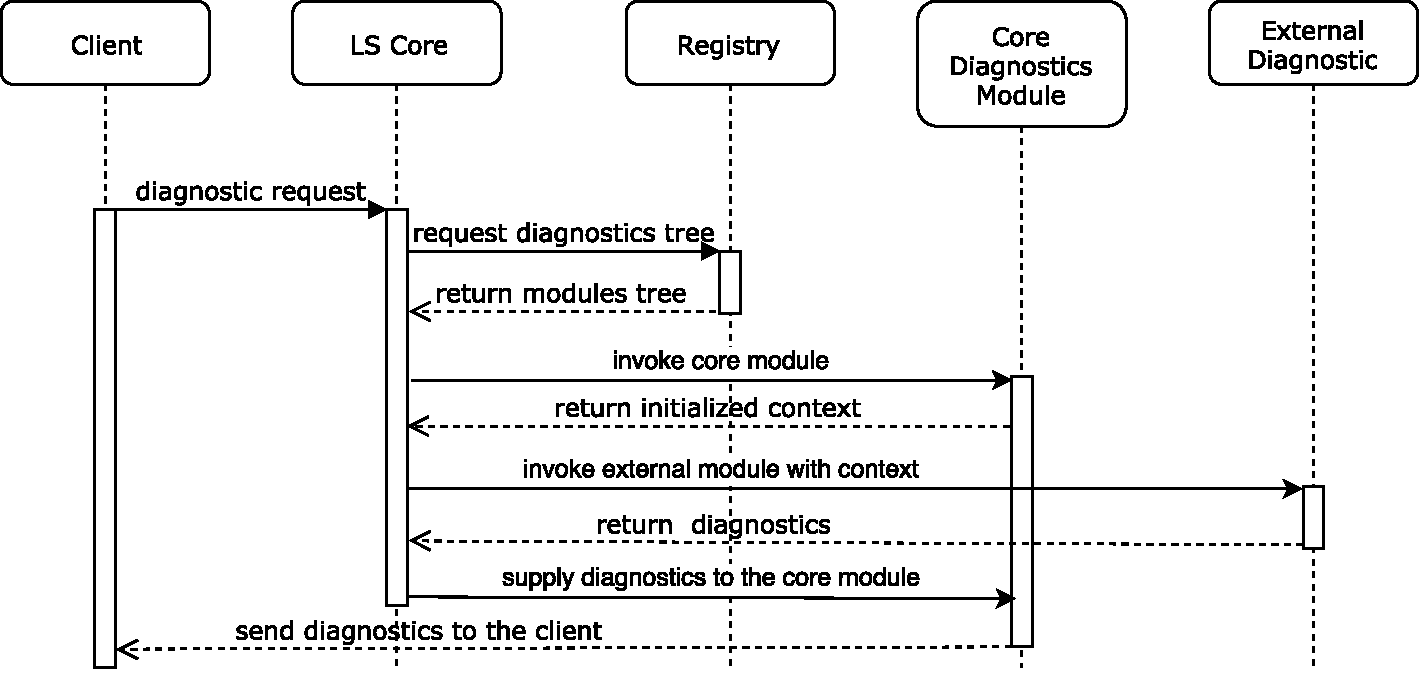
\includegraphics[width=1.0\textwidth]{figs/modules_sd.pdf}
    \caption{Modules invocation sequence diagram}
\end{figure}

Summing up, now we have a way to integrate the compiler into the Language Server, powerful extensible architecture,
that allows to throw in additional functionality for the Language Server, 
and modules hierarchy to start designing the core modules for the Language Server Protocol methods, as well as
the external ones to perform actual analysis and supply Language Server Clients with the code insights.

\section{Development Plan}
To implement a complex system it is vital to split the work into chunks and introduce
the iterative development plan, that would cover a small self-contained part of work on each iteration,
in such a way that the result of each iteration could be presented as a working product.

Also, each iteration should include unit and integration testing to form a good test coverage
at the end of the development process and to simplify project evolution through use of regression testing.

\subsection{A Dummy Language Server}
At first, the very basic functionality will be implemented: 
\begin{itemize}
    \item accepting the connection
    \item handling a diagnostic request with a hardcoded response
\end{itemize}

\begin{figure}[H]
    \centering
    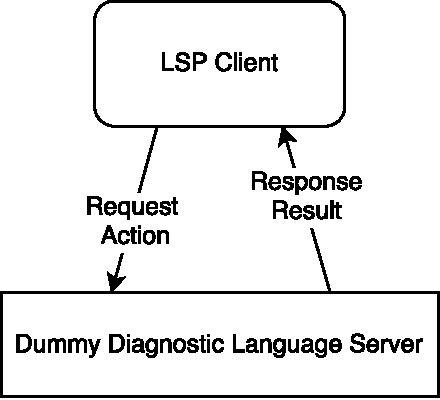
\includegraphics[width=.3\textwidth]{figs/ls_iteration_1.pdf}
    \caption{Iteration 1}
\end{figure}

\newpage
\subsection{SR-driven Language Server}
The next step would be to integrate a compiler and its Semantic Representation
to feature semantic highlights for the SLang Language Server.
\begin{figure}[H]
    \centering
    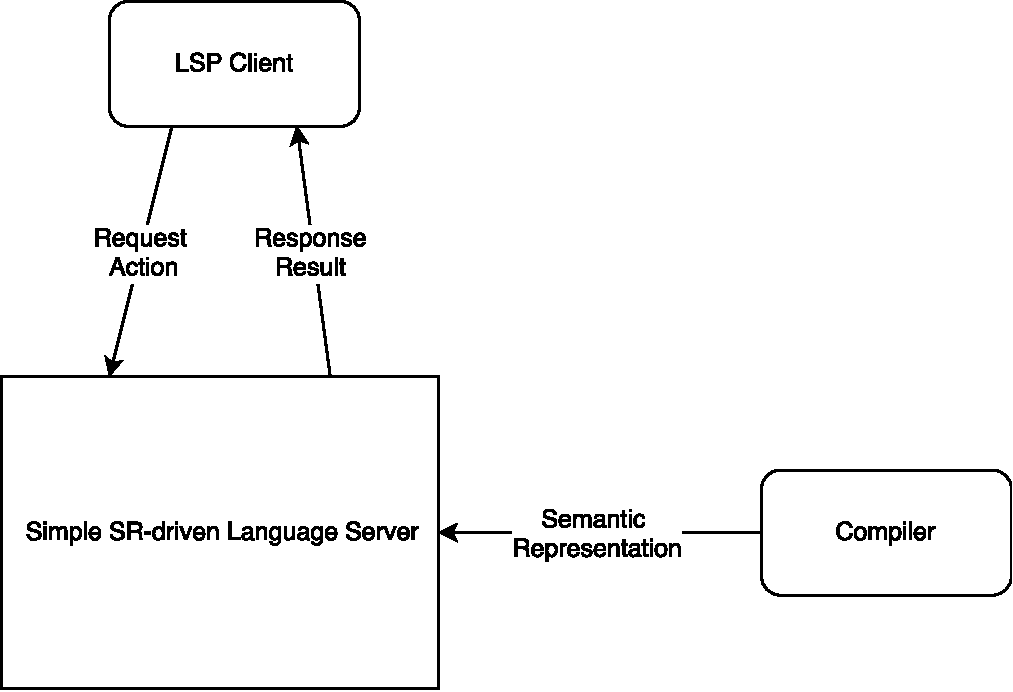
\includegraphics[width=.6\textwidth]{figs/ls_iteration_2.pdf}
    \caption{Iteration 2}
\end{figure}

\subsection{Basic Modular Language Server}
After all the groundwork with the protocol and compiler inter-operation, 
modular architecture implementation may be started: without foreign process extensions for now,
including only built-in modules, that operate in the same address space with the Language Server,
and the simple registry for them, to mock the basement for the future extensible LS.

\begin{figure}[H]
    \centering
    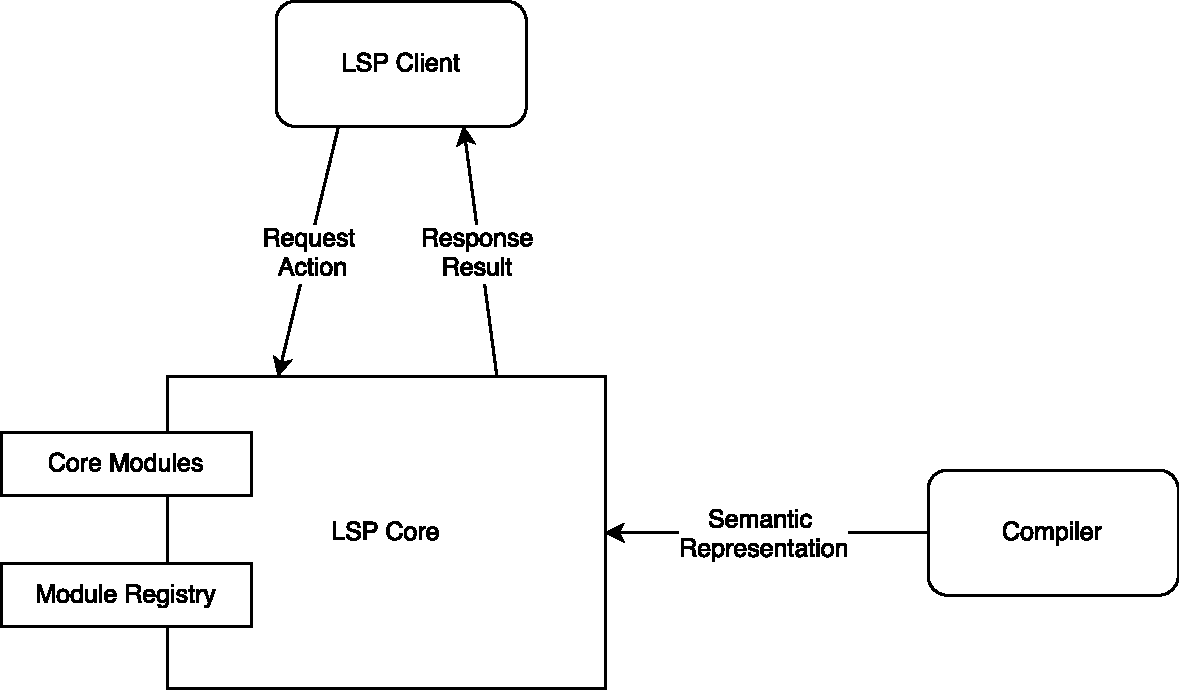
\includegraphics[width=.6\textwidth]{figs/ls_iteration_3.pdf}
    \caption{Iteration 3}
\end{figure}

\subsection{Extensible Language Server}
Finally, the last step will be to extend the registry so it would handle configuration files
and load external modules and to extend the inner protocol and API to work with modules, that are operating
in external processes, thus completing the extensible Language Server implementation for SLang.

\begin{figure}[H]
    \centering
    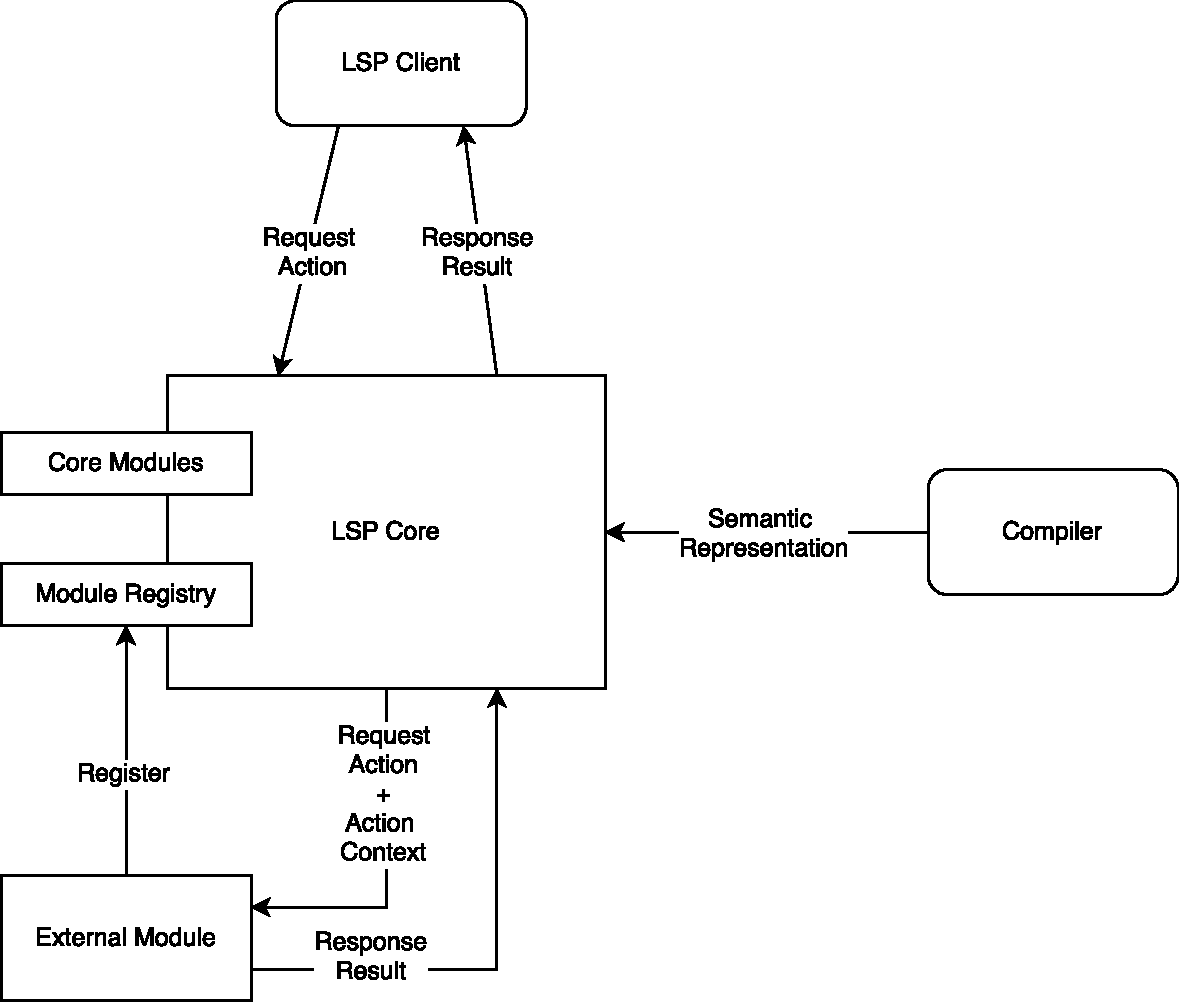
\includegraphics[width=.6\textwidth]{figs/ls_iteration_4.pdf}
    \caption{Iteration 3}
\end{figure}



 


% \section{Basic Language Server Modules}
% \label{sec:met:mods}
% \subsection{Code Semantic Based Highlights Module}
% \label{sec:met:mods:highlights}
% Architecture and methods of IR analysis for highlights

% Mapping from semantic entities to LSP highlighting staff

% \subsection{Autocomplete Module}
% \label{sec:met:mods:autocomplete}
% Description if autocomplete algorithms and data structures choice
\chapter{Implementation}
\label{chap:impl}

\section{Instruments}
\label{sec:impl:instruments}
To not to get drown undertons of work, it was decided to choose an existing OpenSource
Language server as an implementational basis.

As the researcher favourite language is Rust, a modern programming language that aims
to provide zero-cost abstractions, memory and thread safety and blazing speed,
and provide a decent coding experience at the same
the only choice of relatively mature LS for basis is the RLS (Rust Language Server).

After pruning the rust language m dependend code, RLS can speed up implementation process,
as it is equiped with well-tested basic components:
\begin{itemize}
    \item Language Server Protocol implementation
    \item VFS(Virtual File System)
    \item convenient API to accept and dispatch LS messages
\end{itemize}

\subsection{Autocomplete}
\label{sec:impl:ls_mod:autocomplete}
Description if autocomplete implementation

\subsection{Documentation Generator}
\label{sec:impl:ls_mod:docgen}
Description of documentation generation implementation

\section{Language Server control utility\\ library}
\label{sec:impl:ls_control_api}
Testing and Language Server usage as utility outside from within of client-editor Language Server Protocol client would require
a CLI tool, that would be able to act like and aditor and provide an appropriate interface to run single or batch tasks.
\chapter{Evaluation and Discussion}
\label{chap:eval}

Recap of thesis subject

LSP standard complaisance testing

Performance testing

Estimation of developement cost of the full-featured IDE for SLang, comparing that with time and cost of Language Server Implementation

Discussion of future development opportunities

\ldots

\chapter{Conclusion}
\label{chap:conclusion}

Recap

Concluding, the Language Server may be considered to be the most feasible
solution to rapidly bootstrap rich development infrastructure for aspiring new
languages, with a broad path to evolve further.

\ldots


%% REFERENCES
\newpage
\printbibliography

\newpage
\chapter{Appendix A: Trivia}
\label{trivia}

\section{Akkadia: origin of the name}
\label{trivia:akkadia}

\newpage
\thispagestyle{empty}


\begin{titlepage}


\begin{flushleft}
{\Large \bf
Acknowledgements 
}

\vspace{0.01cm}

\rule{\linewidth}{0.05cm}%

\end{flushleft}

{
Acknowledgements \ldots
}

\end{titlepage}

\end{document}
